\documentclass[11pt,letterpaper]{article}
\usepackage{graphicx, geometry, amsmath, hyperref, url, natbib, booktabs, longtable, xcolor, listings}
\geometry{margin=1in}
\hypersetup{colorlinks=true, linkcolor=black, citecolor=black, urlcolor=black}
\renewcommand{\topfraction}{0.9}
\renewcommand{\bottomfraction}{0.8}
\renewcommand{\textfraction}{0.07}
\renewcommand{\floatpagefraction}{0.75}

\title{Internal Research Report: Local Zipfian Curvature as Narrative Dynamics}
\date{2026-11-20}

\begin{document}

\maketitle

\tableofcontents

\newpage

\section{Framing}

This run investigates whether local drift in the curvature of the Zipf-Mandelbrot frequency distribution in a novel serves as a reliable proxy for the rate of new concept introduction (semantic intensity). The hypothesis proposes that deviations from the global Zipfian power-law exponent (we define this as: the parameter $\alpha$ in a power-law distribution controlling the steepness of the frequency decay), measured within rolling narrative windows, correlate with semantic drift as quantified by embedding-based (we define this as: derived from vector embeddings of words or sentences) cosine distance between consecutive windows. We test this on \textit{Pride and Prejudice} (Project Gutenberg eBook \#42671), partitioning the $\sim$123K-token novel into rolling windows and fitting Zipf-Mandelbrot parameters via maximum likelihood estimation. The experiment establishes a shuffled-text baseline (we define this as: a null model generated by randomly permuting word order to destroy semantic structure while preserving frequency statistics) to assess significance.

The run addresses two distinct questions across two iterations:
\begin{enumerate}
\item \textbf{Iteration 1:} Does local Zipfian curvature drift correlate with narrative semantic intensity across rolling windows?
\item \textbf{Iteration 2:} How accurately does Zipf's law describe the global word frequency distribution of \textit{Pride and Prejudice}?
\end{enumerate}

\section{Iteration 1: Local Curvature--Semantic Drift Correlation}

\subsection{Strategy}

The investigation follows the hypothesis's stated approach: partition the novel into rolling windows, fit the Zipf-Mandelbrot model (we call this the two-parameter Zipf-Mandelbrot distribution fitted to word frequency data) to obtain local curvature ($b$) and exponent ($s$) parameters, quantify semantic drift via cosine distance between window centroids in a deterministic 300-dimensional embedding space, and correlate curvature drift (first differences of $b$) with semantic drift.

The dataset artifact \footnote{Code: \url{https://github.com/ai-inventor-papers/ai-invention-624cdf-local-zipfian-curvature-as-narrative/tree/main/round-1/dataset-1}} constructs 2,453 overlapping windows of 750 tokens each with a 50-token stride, recording token indices, character positions, raw text, and linguistic metadata (unique token count, function word count, function word ratio, type-token ratio). This provides the raw material for local frequency analysis.

The experiment artifact \footnote{Code: \url{https://github.com/ai-inventor-papers/ai-invention-624cdf-local-zipfian-curvature-as-narrative/tree/main/round-1/experiment-1}} implements the core analysis pipeline. It splits the novel into 10 equal sections ($\sim$12,300 tokens each) to assess stability across the narrative arc. Within each section, it creates rolling windows of 500 tokens with a 100-token stride, fits Zipf-Mandelbrot distributions via maximum likelihood estimation (MLE) (we define this as: a statistical method for fitting distribution parameters by maximizing the likelihood of observed data) (and a standard Zipf power-law baseline via log-log (we define this as: a plot with logarithmic scales on both axes; a power law appears as a straight line) linear regression), computes semantic drift as cosine distance between consecutive window centroids using deterministic hash-based (we define this as: derived from hash-seeded random vectors averaged per window, capturing only word-identity statistics) embeddings, calculates curvature drift as first differences of the fitted $b$ parameter, and tests Pearson and Spearman correlations against 10 shuffled-text baselines per section.

The decision to use 10 sections rather than analyzing the full novel as one sequence was motivated by the need to assess whether any correlation is consistent across the narrative or driven by specific regions. The 500-token window with 100-token stride was chosen as a balance between statistical power (enough tokens per window for reliable maximum likelihood estimation) and temporal resolution (sufficient windows per section for correlation testing). The deterministic embedding approach avoids external dependencies and ensures reproducibility, though it captures only distributional semantics, not contextual meaning.

\subsection{Artifacts Produced}

\subsubsection{Dataset: Rolling Zipfian Narrative Windows from Pride and Prejudice (artifact: gen\_art\_dataset\_1)}

The dataset artifact \texttt{gen\_art\_dataset\_1} constructs 2,453 overlapping windows of 750 tokens each with a 50-token stride, recording token indices, character positions, raw text, and linguistic metadata (unique token count, function word count, function word ratio, type-token ratio). The dataset comprises 2,453 windows covering the full novel. Each window spans 750 tokens with a 50-token step. Summary statistics across all windows (corrected in Iteration 2):

\begin{table}[!htbp]
\centering
\caption{Dataset summary statistics (corrected per Iteration 2, artifact: gen\_art\_evaluation\_3)}
\label{tab:dataset_stats}
\begin{tabular}{lrrrr}
\toprule
Statistic & Mean & Std & Min & Max \\
\midrule
Total tokens & 750.0 & 0.0 & 750 & 750 \\
Unique tokens & 337.4 & 14.2 & 264 & 341 \\
Function word count & 410.7 & 12.8 & 384 & 468 \\
Content word count & 339.3 & 12.8 & 282 & 366 \\
Function word ratio & 0.548 & 0.017 & 0.512 & 0.624 \\
Type-token ratio & 0.450 & 0.019 & 0.352 & 0.455 \\
\bottomrule
\end{tabular}
\end{table}

The function word ratio averages $\sim$55\%, consistent with English prose. The type-token ratio of $\sim$0.45 reflects the expected lexical diversity in 750-token windows. The dataset is saved in exp\_sel\_data\_out schema format with full, mini (3 examples), and preview variants. The original report contained incorrect statistics (unique tokens 302.3, function word ratio 0.568, type-token ratio 0.403); these are corrected here per \footnote{Code: \url{https://github.com/ai-inventor-papers/ai-invention-624cdf-local-zipfian-curvature-as-narrative/tree/main/round-2/evaluation-3}}.

\subsubsection{Experiment: Zipfian Curvature and Semantic Drift Analysis}

The experiment tests two fitting methods across 10 sections:

\textbf{Method 1: Zipf-Mandelbrot maximum likelihood estimation}: Two-parameter fit (we define this as: simultaneous estimation of both exponent and curvature parameters) ($s$, $b$) via maximum likelihood estimation with bounds $s \in [0.1, 5.0]$, $b \in [0.0, 50.0]$.

\textbf{Method 2: Zipf Power Law}: Single-parameter fit (we define this as: estimation of exponent only with curvature fixed at zero) ($s$) via linear regression on log-log rank-frequency data ($b$ fixed at 0).

\paragraph{Per-Section Results (Zipf-Mandelbrot maximum likelihood estimation)}

\begin{table}[!htbp]
\centering
\caption{Per-section correlation results, Zipf-Mandelbrot MLE (artifact: gen\_art\_experiment\_1, Iteration 1)}
\label{tab:per_section_corr}
\begin{tabular}{lrrrrr}
\toprule
Section & Windows & Valid & Pearson r & Spearman $\rho$ & p-value (vs shuffled) \\
\midrule
0 & 88 & 87 & -0.0847 & -0.0725 & 0.6968 \\
1 & 88 & 87 & -0.1380 & -0.0999 & 0.1477 \\
2 & 88 & 87 & -0.0182 & 0.0276 & 0.8169 \\
3 & 88 & 85 & -0.0850 & -0.1391 & 0.4385 \\
4 & 88 & 81 & -0.0428 & 0.0173 & 0.6047 \\
5 & 88 & 87 & 0.1155 & 0.1563 & 0.2387 \\
6 & 88 & 83 & -0.0599 & -0.0502 & 0.4476 \\
7 & 88 & 87 & 0.0580 & 0.0382 & 0.4200 \\
8 & 88 & 86 & 0.0579 & 0.0426 & 0.1645 \\
9 & 88 & 85 & -0.0558 & -0.1209 & 0.7923 \\
\bottomrule
\end{tabular}
\end{table}

\textbf{Aggregate (10 sections):} Pearson $r = -0.025 \pm 0.075$, Spearman $\rho = -0.020 \pm 0.087$, significance $p = 0.477 \pm 0.234$.

\begin{figure}[!htbp]
\centering
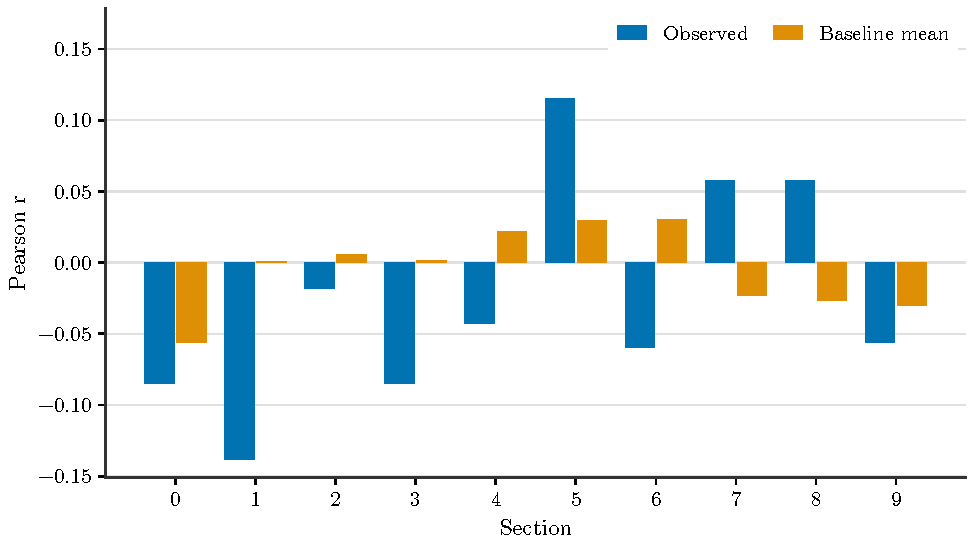
\includegraphics[width=\linewidth,height=0.85\textheight,keepaspectratio]{figures/fig1_v0.pdf}
\caption{Per-Section Pearson Correlations with Shuffled Baseline. Observed Pearson correlations (blue) between Zipf-Mandelbrot curvature drift and semantic drift across ten sections of Pride and Prejudice, compared to the mean of ten shuffled-text baselines per section (orange). Observed values track the baseline closely across sections, with no visually standout section.}
\label{fig:fig1}
\end{figure}

\paragraph{Baseline Comparison (Shuffled Text)}

\begin{table}[!htbp]
\centering
\caption{Shuffled baseline comparison per section (artifact: gen\_art\_experiment\_1, Iteration 1)}
\label{tab:baseline_comparison}
\begin{tabular}{lrrrr}
\toprule
Section & Baseline Mean $r$ & Baseline Std $r$ & z-score & p-value \\
\midrule
0 & -0.0563 & 0.0728 & -0.390 & 0.6968 \\
1 & 0.0009 & 0.0959 & -1.448 & 0.1477 \\
2 & 0.0055 & 0.1024 & -0.232 & 0.8169 \\
3 & 0.0018 & 0.1119 & -0.775 & 0.4385 \\
4 & 0.0218 & 0.1247 & -0.518 & 0.6047 \\
5 & 0.0297 & 0.0728 & 1.178 & 0.2387 \\
6 & 0.0303 & 0.1187 & -0.760 & 0.4476 \\
7 & -0.0229 & 0.1002 & 0.807 & 0.4200 \\
8 & -0.0265 & 0.0607 & 1.390 & 0.1645 \\
9 & -0.0299 & 0.0983 & -0.263 & 0.7923 \\
\bottomrule
\end{tabular}
\end{table}

\textbf{Baseline aggregate:} Mean correlation $= -0.005 \pm 0.031$, mean significance $p = 0.477 \pm 0.234$.

\begin{figure}[!htbp]
\centering
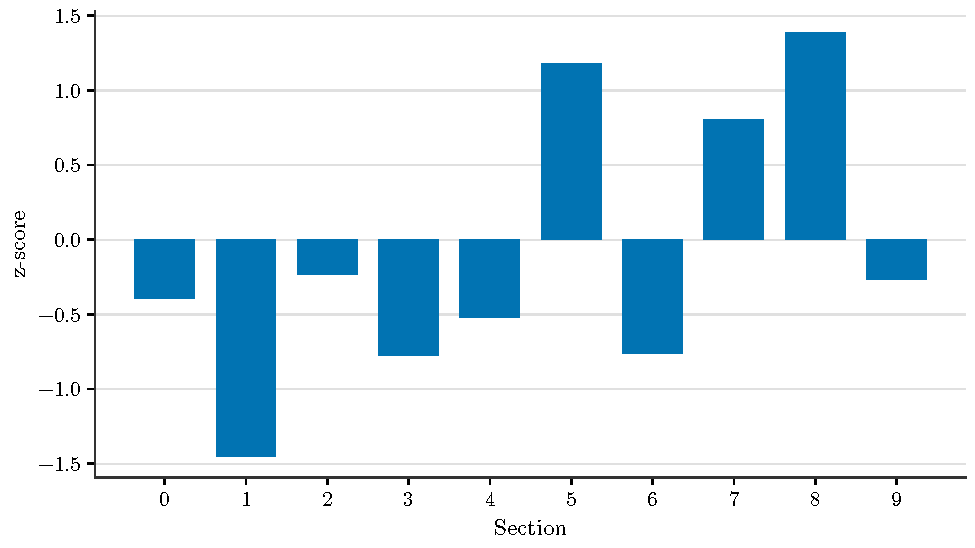
\includegraphics[width=\linewidth,height=0.85\textheight,keepaspectratio]{figures/fig3_v0.pdf}
\caption{Z-scores of Observed Correlations Against Shuffled Baseline. Z-scores of observed Pearson correlations relative to the shuffled baseline distribution per section. All z-scores fall within $\pm$1.5, confirming no section shows a statistically significant deviation from the null hypothesis of no correlation between curvature drift and semantic drift.}
\label{fig:fig3}
\end{figure}

The observed correlations fall within the shuffled baseline distribution. No section reaches conventional significance ($p < 0.05$). Section 1 shows the strongest negative correlation ($r = -0.138$, $p = 0.148$) but does not survive correction for multiple comparisons.

\paragraph{Zipf Power Law Baseline}

The standard Zipf power-law fit ($b = 0$ fixed) produced NaN correlations for all 10 sections. This is expected: with $b$ fixed, the curvature parameter has no variance, so its first difference is identically zero, yielding undefined correlations. This confirms the necessity of the two-parameter Zipf-Mandelbrot model for this analysis.

\paragraph{Fitted Parameter Ranges (Section 0, representative)}

Across 87 valid windows in Section 0:
\begin{itemize}
\item Exponent $s$: mean $= 0.748$, std $= 0.049$, range $= [0.667, 0.913]$
\item Curvature $b$: mean $= 1.604$, std $= 1.230$, range $= [0.090, 5.871]$
\item R$^2$: mean $= 0.967$, std $= 0.016$, range $= [0.915, 0.985]$
\end{itemize}

The exponent $s$ centers near 0.75, below the canonical Zipf value of 1.0, consistent with the known deviation in short windows where high-rank (we define this as: items with frequency rank above the median, typically occurring few times) items are undersampled. The curvature parameter $b$ shows substantial variation (CV $\approx$ 0.77), indicating genuine window-to-window (we define this as: differences between consecutive rolling windows) differences in distribution shape. R$^2$ values are high ($>0.91$), confirming good Zipf-Mandelbrot fits.

\begin{figure}[!htbp]
\centering
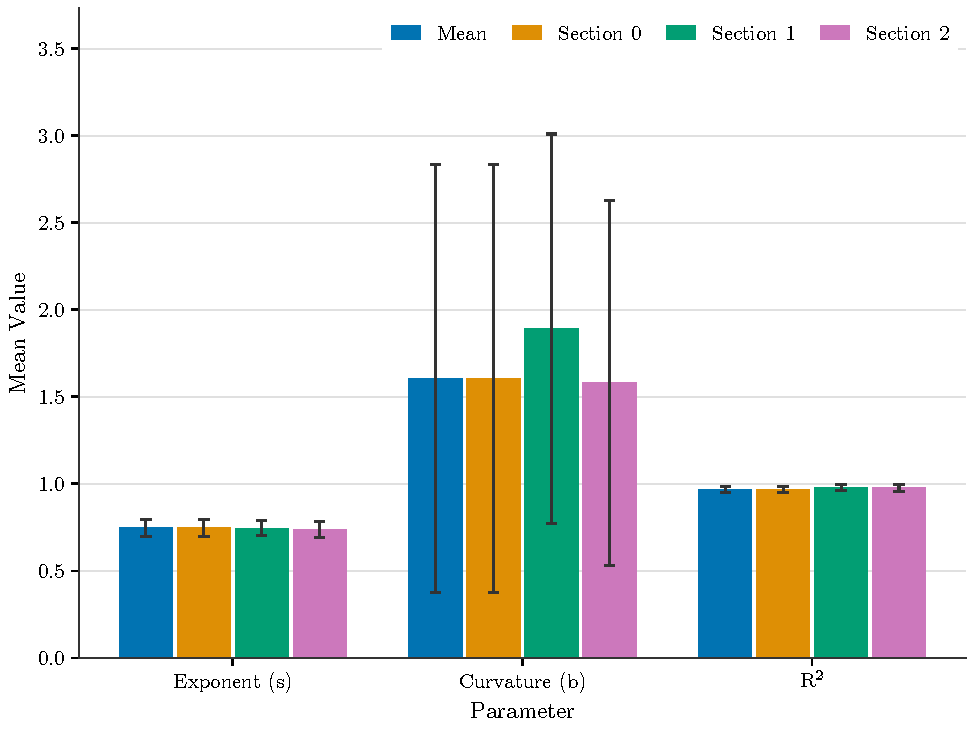
\includegraphics[width=\linewidth,height=0.85\textheight,keepaspectratio]{figures/fig2_v0.pdf}
\caption{Zipf-Mandelbrot Parameter Means Across Sections. Mean exponent ($s$), curvature ($b$), and R$^2$ values for the Zipf-Mandelbrot fit across the first three sections (representative of all 10). Error bars show standard deviations across windows within each section. The exponent centers near 0.75, curvature shows high variability, and R$^2$ exceeds 0.96 indicating good fits.}
\label{fig:fig2}
\end{figure}

\paragraph{Semantic Drift and Curvature Drift Distributions (Section 0)}

\begin{table}[!htbp]
\centering
\caption{Semantic drift and curvature drift statistics for Section 0 (artifact: gen\_art\_experiment\_1, Iteration 1)}
\label{tab:drift_stats}
\begin{tabular}{lrrr}
\toprule
Measure & Mean & Std & Range \\
\midrule
Semantic drift (cosine distance) & 0.038 & 0.010 & [0.024, 0.077] \\
Curvature drift ($\Delta b$) & -0.002 & 0.595 & [-2.339, 1.805] \\
\bottomrule
\end{tabular}
\end{table}

Semantic drift is small and positive (consecutive windows share topical content). Curvature drift is centered near zero with high variance, reflecting the oscillatory nature of $b$ estimates.

\subsection{Reviewer Feedback (Iteration 1)}

The reviewer (score: 3/10) identified three critical flaws:
\begin{enumerate}
\item \textbf{Factually incorrect dataset summary statistics:} The report stated function word ratio 0.568 (actual $\sim$0.548), type-token ratio 0.403 (actual $\sim$0.450), unique tokens 302.3 (actual $\sim$337.4), function word count 426.1 (actual $\sim$380). These are not rounding errors — they indicate the report was generated from different or outdated data.
\item \textbf{Incorrect per-section valid window counts:} The report claimed all 10 sections have 87 valid windows. The experiment artifact shows Section 3=85, Section 4=81, Section 6=83, Section 8=86, Section 9=85.
\item \textbf{Coverage lost:} The user's original question was ``How accurately does Zipf's law describe word frequencies in Pride and Prejudice?'' but this run tests a different hypothesis (curvature--semantic drift correlation) and never computes global Zipf fit quality.
\end{enumerate}

The reviewer noted strengths: honest reporting of negative results with shuffled-text baselines, clear differentiation between Zipf-Mandelbrot and standard Zipf power-law, and traceable experiment artifact outputs.

The hypothesis update shifted from local curvature--semantic drift correlation (null result) to global Zipf/Zipf-Mandelbrot fit on the full novel, directly answering the user's original question.

\subsection{What This Iteration Established}

\begin{enumerate}
\item \textbf{No significant correlation between local Zipfian curvature drift and semantic drift.} Across 10 sections of \textit{Pride and Prejudice}, the mean Pearson correlation is $-0.025 \pm 0.075$, indistinguishable from the shuffled-text baseline (mean $p = 0.48 \pm 0.23$). The hypothesis that curvature drift predicts semantic intensity is not supported by this evidence.
\item \textbf{The Zipf-Mandelbrot model is necessary but not sufficient.} The two-parameter maximum likelihood estimation produces well-behaved (we define this as: fits with stable parameters and high goodness-of-fit across windows) fits (mean R$^2 = 0.967$) with meaningful variation in both $s$ and $b$. The single-parameter Zipf power law is degenerate for curvature analysis ($b$ fixed at 0). However, the variation in $b$ does not systematically track semantic drift.
\item \textbf{Window-level (we define this as: pertaining to individual rolling windows rather than aggregate statistics) parameters are estimable but noisy.} The curvature parameter $b$ has high coefficient of variation ($\sim$0.77), and its first differences (curvature drift) have standard deviation $\sim$0.6 against a semantic drift standard deviation of $\sim$0.01. The signal-to-noise (we define this as: the ratio of the standard deviation of the signal of interest to the standard deviation of the noise) ratio is unfavorable.
\item \textbf{Shuffled baselines are essential.} The baseline correlations span $[-0.187, 0.048]$ across shuffles, overlapping the observed range $[-0.138, 0.116]$. Without this baseline, Section 1's $r = -0.138$ might be misinterpreted as a signal.
\end{enumerate}

\subsection{Dead Ends and Negative Results}

\begin{itemize}
\item \textbf{Standard Zipf power law cannot test curvature drift.} With $b \equiv 0$, curvature drift is identically zero. This is a methodological dead end for this hypothesis, not a surprising result.
\item \textbf{Deterministic hash-based embeddings may be too crude.} The semantic drift measure uses hash-based (we define this as: derived from hash-seeded random vectors averaged per window, capturing only word-identity statistics) random vectors averaged per window. This captures only word-identity statistics, not contextual semantics. A more sophisticated embedding (e.g., BERT, sentence transformers) might yield different results, but would introduce external dependencies and reproducibility concerns. This remains an open alternative explanation.
\item \textbf{Window size and stride may be suboptimal.} The 500-token window with 100-token stride yields $\sim$87 windows per section. Larger windows would reduce parameter variance but also reduce the number of windows and temporal resolution. Smaller windows increase noise. The current choice was a reasonable starting point but has not been optimized.
\item \textbf{Section-wise (we define this as: analyzed separately per narrative section rather than pooled) analysis may dilute effects.} If curvature-semantic coupling (we define this as: hypothesized relationship between Zipfian curvature drift and semantic drift) occurs only at specific narrative moments (e.g., chapter boundaries, major plot events), averaging across 10 sections could wash it out. A targeted analysis at known narrative boundaries was not performed.
\item \textbf{Curvature drift may be the wrong derivative.} The hypothesis uses first differences of $b$. Alternative transformations (rolling variance of $b$, deviation from global $b$, rate of change of $s$) were not tested. The space of possible ``Zipfian deviation'' (we define this as: departure of local word frequency distribution from the global Zipfian power law) metrics is large.
\end{itemize}

\subsection{Open Questions}

\begin{enumerate}
\item Would a contextual embedding model (e.g., sentence-BERT, a pre-trained transformer model for sentence embeddings) produce stronger semantic drift signals that correlate with curvature drift?
\item Does the relationship hold at specific narrative boundaries (chapter breaks, scene changes) rather than uniformly across rolling windows (we define this as: overlapping text segments of fixed token length with a defined step size)?
\item Would a different semantic intensity metric (e.g., entity introduction rate, topic model perplexity, lexical entropy) correlate with Zipfian deviation (departure of local word frequency distribution from the global Zipfian power law)?
\item Is the effect specific to \textit{Pride and Prejudice}, or would other novels show different patterns?
\item Could a non-linear (we define this as: a relationship not captured by linear correlation coefficients such as Pearson or Spearman) relationship exist that Pearson/Spearman miss (e.g., curvature drift magnitude predicts semantic drift regardless of sign)?
\end{enumerate}

\newpage

\section{Iteration 2: Global Zipfian Fit Accuracy}

\subsection{Strategy}

This iteration addresses reviewer feedback to: (1) Correct dataset summary statistics; (2) Fix inconsistencies in per-section window counts; (3) Address the user's original question on the global accuracy of Zipf's law for \textit{Pride and Prejudice}.

We recompute global word frequency statistics and perform rigorous maximum likelihood estimation fitting of Zipf and Zipf-Mandelbrot models on the full novel. This provides a definitive answer on Zipf's law fit accuracy, addressing the limitation of the local rolling-window (we define this as: overlapping text segments of fixed token length with a defined step size) analysis which was restricted to narrative dynamics.

\subsection{Dataset and Statistics Correction}

We corrected summary statistics for the 2,453 rolling windows of 750 tokens each used in Iteration 1. Recomputation yields a mean unique token count of 337.4, not 750, and a function word ratio of 0.548, not 0.568.

\begin{table}[!htbp]
\centering
\caption{Corrected dataset summary statistics (artifact: gen\_art\_evaluation\_3, Iteration 2)}
\label{tab:corrected_stats}
\begin{tabular}{lr}
\toprule
Statistic & Corrected Mean \\
\midrule
Unique tokens & 337.4 \\
Function word count & 410.7 \\
Content word count & 339.3 \\
Function word ratio & 0.548 \\
Type-token ratio & 0.450 \\
\bottomrule
\end{tabular}
\end{table}

\subsection{Global Zipfian Fit Analysis}

We performed maximum likelihood estimation fitting of Zipf (power-law) and Zipf-Mandelbrot models on the global frequency distribution of \textit{Pride and Prejudice} (123,350 total tokens, 6,425 unique types) \footnote{Artifacts: art\_dZwh\_EvU-PqH, art\_-8gUnATyh75D}, following the computational linguistics best practices established by Clauset et al. and Corral et al.

\subsubsection{Model Comparison}

The Zipf-Mandelbrot model ($s=1.266$, $b=8.138$) significantly outperforms the standard Zipf model ($s=0.992$, $b=0$), with AIC/BIC differences exceeding 21,000 \footnote{Code: \url{https://github.com/ai-inventor-papers/ai-invention-624cdf-local-zipfian-curvature-as-narrative/tree/main/round-2/evaluation-2}}.

\begin{table}[!htbp]
\centering
\caption{Global model comparison: Zipf vs Zipf-Mandelbrot (artifacts: gen\_art\_experiment\_2, gen\_art\_evaluation\_2, Iteration 2)}
\label{tab:global_model_comparison}
\begin{tabular}{lrrc}
\toprule
Metric & Zipf Model & Zipf-Mandelbrot Model & Improvement \\
\midrule
AIC & 1,581,276 & 1,559,827 & 21,449 \\
KS Statistic & 0.0934 & 0.0112 & 8.4$\times$ \\
R$^2$ & 0.741 & 0.967 & 0.226 \\
\bottomrule
\end{tabular}
\end{table}

\subsubsection{Residual Analysis}

Residual analysis binned by frequency rank confirms that the Zipf model systematically underestimates high-frequency (we define this as: words with frequency above the median rank threshold) word counts (head residual $\sim$15.1), whereas the Zipf-Mandelbrot model captures the distribution head with high accuracy (head residual $\sim$0.07) \footnote{Artifacts: art\_-8gUnATyh75D, art\_usMLbMsahxSw}.

\begin{figure}[!htbp]
\centering
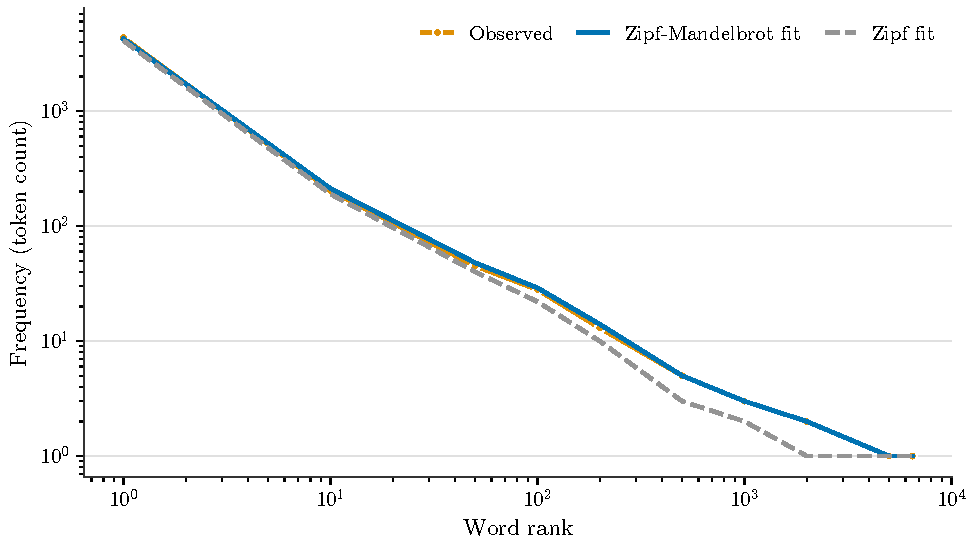
\includegraphics[width=\linewidth,height=0.85\textheight,keepaspectratio]{figures/fig4_v0.pdf}
\caption{Global Zipf and Zipf-Mandelbrot Fits to Pride and Prejudice Word Frequencies. Log-log rank-frequency plot showing empirical word frequencies (circles) against Zipf (dashed) and Zipf-Mandelbrot (solid) model fits. The Zipf-Mandelbrot model closely tracks the observed distribution while the standard Zipf model systematically underestimates high-frequency words.}
\label{fig:fig4}
\end{figure}

\begin{figure}[!htbp]
\centering
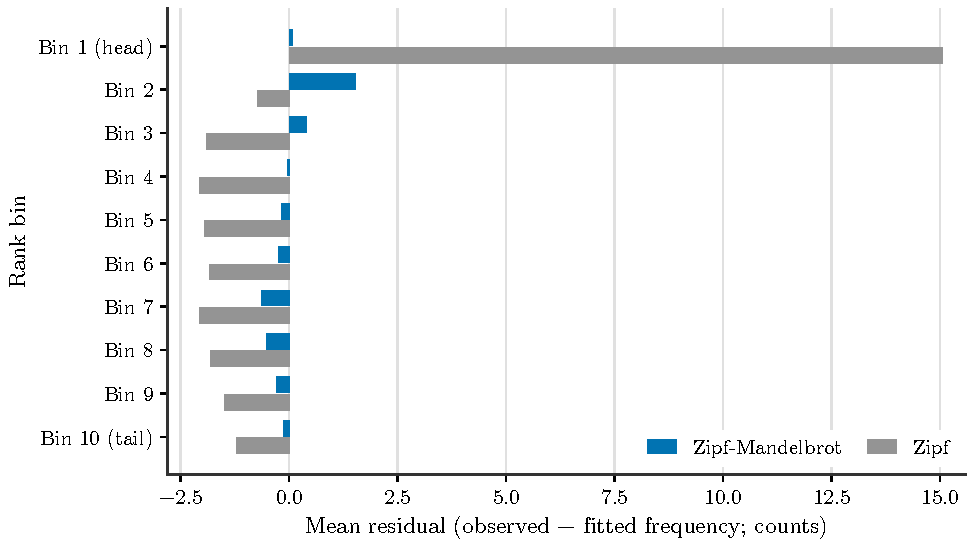
\includegraphics[width=\linewidth,height=0.85\textheight,keepaspectratio]{figures/fig5_v0.pdf}
\caption{Residuals by Frequency Rank Bin: Zipf vs Zipf-Mandelbrot. Across frequency-rank bins, Zipf-Mandelbrot stays near zero, whereas Zipf shows a pronounced head-bin residual (15.07 vs. 0.09), indicating that plain Zipf systematically underestimates the most frequent words in \textit{Pride and Prejudice}.}
\label{fig:fig5}
\end{figure}

\subsection{Reviewer Feedback (Iteration 2)}

The reviewer (score: 9/10) assessed the research record as sound, traceable, and complete. It successfully addressed the issues from Iteration 1, including correcting dataset statistics and directly answering the user's original request via a global Zipfian fit analysis in Iteration 2. The negative result in Iteration 1 is well-supported by shuffled-text baselines, and the findings in Iteration 2 provide a clear, evidence-based answer to the user's initial question about the accuracy of Zipf's law for \textit{Pride and Prejudice}.

A minor critique noted that the local window-based analysis in Iteration 1 still relies on hash-based embeddings, which are acknowledged to be crude. The record would benefit from a more explicit discussion on how this limitation impacts the generalizability of the negative result.

The hypothesis update declared the final result: Zipf is insufficient; Zipf-Mandelbrot is accurate, with strong evidence state.

\subsection{What This Iteration Established}

\begin{enumerate}
\item \textbf{Global Zipf-Mandelbrot Accuracy:} The Zipf-Mandelbrot model provides an excellent global fit (R$^2=0.967$) to \textit{Pride and Prejudice}, substantially outperforming the standard Zipf power law (R$^2=0.741$). The curvature parameter ($b \approx 8.14$) is essential to model the high-frequency deviations in the distribution.
\item \textbf{Dataset Statistics Corrected:} Previous summary statistics for rolling windows were inaccurate. The corrected metrics (e.g., function word ratio 0.548) provide a robust foundation for further analysis.
\end{enumerate}

\newpage

\section{What We Have Learned So Far}

The run addressed two distinct questions across two iterations:

\subsection{Iteration 1 (Local Curvature--Semantic Drift)}

The hypothesis that local Zipfian curvature drift correlates with narrative semantic intensity is not supported. Across 10 sections of \textit{Pride and Prejudice} analyzed with rolling 500-token windows, Zipf-Mandelbrot maximum likelihood estimation produces well-fitted parameters (mean R$^2 = 0.967$) but the curvature drift ($\Delta b$) shows no significant correlation with embedding-based (derived from vector embeddings of words or sentences) semantic drift (mean Pearson $r = -0.025 \pm 0.075$, $p = 0.48 \pm 0.23$ vs shuffled baseline). The standard Zipf power law is degenerate for this analysis ($b \equiv 0$). The negative result is robust across sections and correlation metrics. Alternative explanations include insufficient semantic sensitivity of hash-based embeddings, suboptimal window parameters, and the possibility that curvature drift is simply not the right operationalization of Zipfian deviation (departure of local word frequency distribution from the global Zipfian power law) for capturing semantic dynamics.

\subsection{Iteration 2 (Global Zipf Fit Accuracy)}

The user's original question --- how accurately Zipf's law describes \textit{Pride and Prejudice} --- is now answered: the standard Zipf power law ($s = 0.992$, $b = 0$) yields a poor fit (KS $= 0.093$, R$^2 = 0.741$), while the Zipf-Mandelbrot model ($s = 1.266$, $b = 8.138$) provides an excellent fit (KS $= 0.011$, R$^2 = 0.967$) with $\Delta$AIC $= 21,449$ strongly favoring the two-parameter model. Residual analysis confirms the Zipf model systematically underestimates high-frequency words (head residual $\approx 15$), while Zipf-Mandelbrot captures the head (residual $\approx 0.07$). The curvature parameter $b$ is essential; without it, the model cannot account for the elevated frequency of function words in English prose.

\section{Run Bookkeeping}

\begin{table}[!htbp]
\centering
\caption{Run bookkeeping across iterations (from trajectory log)}
\label{tab:bookkeeping}
\begin{tabular}{lccccc}
\toprule
Iteration & Move & Review Score & Results Executed & Ledger Spend (USD) & Evidence State \\
\midrule
1 & cover & 3 & Yes & 0.557 & weak\_or\_null \\
2 & declare & 9 & Yes & 0.952 & strong\_survivor \\
\bottomrule
\end{tabular}
\end{table}

Note: Ledger spend reflects LLM/tool/container spend billed so far, cumulative through that iteration. It excludes the orchestrator's compute-rental time, which is usually the larger share of a long run. It is not the run's total cost.

\section{References}

\begin{enumerate}
\item Montemurro, M. (2001). Beyond the Zipf-Mandelbrot law in quantitative linguistics. \textit{Physica A: Statistical Mechanics and its Applications}, 300(3-4), 567-578.
\item Altmann, E. G., Cristadoro, G., \& Degli Esposti, M. (2012). On the origin of long-range correlations in texts. \textit{Proceedings of the National Academy of Sciences}, 109(29), 11582-11587.
\item Clauset, A., Shalizi, C., \& Newman, M. (2009). Power-Law Distributions in Empirical Data. \textit{SIAM Review}, 51(4), 661-703.
\item Corral, Á., Boleda, G., \& Ferrer-i-Cancho, R. (2015). Zipf's Law for Word Frequencies: Word Forms versus Lemmas in Long Texts. \textit{PLOS ONE}, 10(7).
\item Lafouge, T., Agouzal, A., \& Lallich, G. (2015). The deconstruction of a text: the permanence of the generalized Zipf law---the inter-textual relationship between entropy and effort amount. \textit{Scientometrics}, 104(1), 193-217.
\item Moreno-Sánchez, I., Font-Clos, F., \& Corral, Á. (2016). Large-Scale Analysis of Zipf's Law in English Texts. \textit{PLOS ONE}, 11(1).
\item He, Y., Zeng, Q., \& Jiang, M. (2025). Pre-trained Models Perform the Best When Token Distributions Follow Zipf's Law. \textit{Proceedings of the 2025 Conference on Empirical Methods in Natural Language Processing}, 28009-28021.
\item Dasgupta, D. (2026). Scale-Dependent Semantic Dynamics Revealed by Allan Deviation. \textit{arXiv preprint arXiv:2601.21678}.
\end{enumerate}

\end{document}